\chapter{Cost/benefit analysis}

\section{Introduction}\label{lesson-3-introduction}

\emph{Why a company or public institution would base its strategy on FLOSS ?} With this initial question we led the argument that a company would gain by associating their business model to FLOSS projects 

Most companies are interested in products not if its FLOSS or not. A company wants the service and doesn't care about its origin, in most cases. Wants the fiability and consistence of the product that are buying. At the other hand we have integration companies that are near to FLOSS products development that allows them a deeper analysis capabilities.

\subsection{Cost/benefit analysis}\label{lesson-3-cost-benefit}

We present an analysis of costs / benefits related to FLOSS products shown on consistency beyond the brand name starting with one sentence: \emph{FLOSS projects are available to anyone with a computer and an internet connection}.

\begin{enumerate}

    \item Advantages of public scrutiny and chances for improvements
    \begin{itemize}
        \item Compare benchmarks between projects and its goals. Could analyse every code line as you want and check every feature that has the product and compare with other projects using standar quality models\footnote{QSOS, OpenBRR, QUALOSS} adapted to your interests. And of course, anyone can view the source code of your project so you have to get it right and well documentated.
    \end{itemize}

    \item Real competition in development and maintenance
    \begin{itemize}
        \item In private projects there is only a main company that could develop improvements in software. Maintenance is very important and every new business model could grow around FLOSS projects. So your product as a costumer depends only of one company, what would happen if the company goes bankrupt?
    \end{itemize}

    \item Technical feasibility vs. marketing
    \begin{itemize}
        \item Its technical feasibility is its own marketing. Private Software only has its own reports about its software, so you only could trust them without any test. In some cases, allowed some evidence but you can not be sure that what you are testing is the final product so you are limited by what the company offers. Choose before (private) or after (free) the trial.
    \end{itemize}

    \item Easy testing, deployment, update
    \begin{itemize}
        \item Easy update to continue retrieving improvements. If the product is FLOSS you can update, test and deploy yourself the product because you have all needed tools, source code. Of course you can pay another company for develop updates in the product too and continue focused in your issues.
    \end{itemize}

    \item Lower barriers to business opportunities
    \begin{itemize}
        \item Infraestructure around FLOSS is cheaper and lets you focus in your own business. Lets you focus only in your business niche. If you need to add something that could be interesting to your model you can include your goals in FLOSS Roadmaps, it's not easy but it's possible despite in the private roadmaps solutions. FLOSS products gives you easy technology access.
    \end{itemize}

    \item Non-formal collaboration and pooling of resources
    \begin{itemize}
        \item FLOSS projects could have competitors working together in the project. As an example we have AMD and Intel working together in Linux even Microsoft for first time\footnote{http://www.linuxfoundation.org/news-media/announcements/2012/04/linux-foundation-releases-annual-linux-development-report}. Google and Apple contribute with Webkit as main companies\footnote{http://trac.webkit.org/wiki/WebKit\%20Team}. Because of community rules and make a common infraestructure for all. NDA doesn't exist.
    \end{itemize}

    \item Technology transfer
    \begin{itemize}
        \item Low barriers to share knowledgement. Web is used as a tool thanks to FLOSS communities. \emph{if each one has an apple and we exchange apples we still have each but if we each have an idea and we exchange, the two will have two ideas.}
    \end{itemize}

    \item Libre software as an strategic tool
    \begin{itemize}
        \item FLOSS as part of your strategy. Use FLOSS products to reach to your desired business niche, as a tool to easily reach your goals. We have the sample of Google that wants advertisement benefits in mobiles and used FLOSS (Android) to achieve its goal in mobile market to make people use their services easily.
    \end{itemize}

\end{enumerate}

\section{What disappears when a business uses libre software?}\label{lesson-3-disappears}

What brings us to a business using FLOSS technologies? What doors are open to us?

\begin{itemize}
    \item \emph{Dependence on monopolies:}
    \begin{itemize}
        \item Real competition, better products, better services. The technology is not dependent on a single supplier, technology is the union of different suppliers in oneself when using the product, it can become a provider of the same technology.
    \end{itemize}  
    \item \emph{Importance of vendor reliability:}
    \begin{itemize}
        \item Future depends on product acceptance in the market. The vendor is exposed to continuous product analysis by different users. In every field of use of the product are certain tests that help the overall assessment and therefore the acceptance thereof by users. This process causes the provider to increase its reliability with regard to the consumer.
    \end{itemize}  
    \item \emph{Decisions taken based on few elements:}
    \begin{itemize}
        \item Software can be tested in its real environment, at a very low cost. You have the possibility to imagine all kind of test in every environment you choose to check product capabilities and compare your results with other analysis.
    \end{itemize}  
    \item \emph{Dependence on the strategy of providers:}
    \begin{itemize}
        \item Decisions on the evolution of a product taken for those contributing with resources. You have the possibility to include your thought into the product roadmap, also you can improve with your contributions to the project and share ideas with the community in an cross-ideas open platform.
    \end{itemize}  
    \item \emph{Confidence on "black boxes":}
    \begin{itemize}
        \item Using FLOSS projects we can see the whole process of the data inside de technology, we don't have \emph{black holes} where we miss which operations are done. We do not lose the path of process operations being applied to our data the software from input to output. For example an application service like gmail. This application hides we treat our data to drive the process of sending an email and the result shows that message has been sent as output  
    \end{itemize}  
   
\end{itemize}

\pagebreak

    \begin{figure}[h]
        \begin{center}
            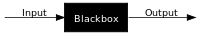
\includegraphics{blackbox}
            \caption[BlackBox]{BlackBox; we only can see the input and the output, not the process.}
            \label{fig:blackbox}
        \end{center}
    \end{figure}



\section{Conclusions}\label{lesson-3-conclusions}

\textbf{TBC}
